\section{Образование химической связи между атомами. Ковалентная связь. Валентность. Правило октета. Формальный заряд и степень окисления элемента в соединении.}

Свободные атомы большинства элементов стремятся объединяться друг с другом, образуя системы с более низкой энергией — молекулы, цепи, слои, каркасы. Здесь будем в основном говорить о молекулах, все остальное больше касается органики.

\textbf{Молекула} --- устойчивая электронейтральная частица, представляющая собой мельчайшую частицу вещества, обладающую его химическими свойствами.

\subsection{Ковалентная связь}

Подобная связь между атомами называется \textbf{химической связью}, которая имеет электростатическую природу (основана на электростатической связи между ядрами и электронами). Атомные химические связи обычно делятся на \textit{ионные}, \textit{ковалентные} и \textit{металлические}. Химические связи также могут возникать при сближении молекул (тогда это межмолекулярные связи), однако такие связи гораздо слабее атомных. При разрыве межмолекулярных связей изменяются не сами вещества, а лишь, например, их агрегатное состояние.

Ковалентная связь --- связь, возникающая при перекрывании электронных орбиталей двух атомов и последующем объединении пар электроном (создании обобщенной электронной пары) [согласно методу валентных связей].

Известно два механизма образования такой связи: либо оба взаимодействующих атома предоставляют в общее пользование для пары по одному электрону, либо же один атом (донор) предоставляет пару электронов, а второй (акцептор) --- пустую орбиталь для этой пары. Последний механизм называется \textbf{донорно-акцепторным}. Результат, независимо от механизма, одинаковый: две орбитали перекрываются, на них оказываются два электрона. бывает и такое, что работают оба механизма. Например, в ионе аммония \ce{NH4+} три связи образуются перекрыванием одноэлектронных облаков, а одна --- по донорно-акцепторному механизму. Связи при этом между собой неразличимы и равноценны.

\subsection{Валентность}

\textbf{Валентность} --- численная характеристика способности атомов элемента соединяться с определенным число атомов других элементов. Значение указывают (если указывают) римскими цифрами. За единицу валентности принята валентность атомов водорода. Валентность атома элемента в его водородном соединении равна числу атомов водорода в молекуле.

Некоторые элементы имеют постоянную валентность (например, \ce{H}[\RN{1}], \ce{O}[\RN{2}], \ce{Al}[\RN{3}] и т.д.), некоторые же (большинство) имеют переменную валентность (например, \ce{N}[\RN{1}, \RN{2}, \RN{3}, \RN{4}, \RN{5}]).

Для объяснения причин появления ковалентных связей в свое время Г.Н. Льюисом было предложено так называемое \textbf{правило октета}, согласно которому при образовании молекул атомы удовлетворяют свою потребность в достижении 8-электронной валентной оболочки, которая подобная электронной конфигурации благородных газов. Происходит это как раз за счет попарного обобществления валентных электронов.

\subsection{Степень окисления элемента}

\textbf{Степень окисления атома} есть численная величина электрического заряда, приписываемого атому в предположении, что соединение состоит исключительно из ионов. В случае ковалентной связи между одинаковыми атомами электроны делят между атомами поровну. Степень окисления указывается справа сверху от символа элемента в порядке: знак, численное значение (например, \ce{H2^+S^{+6}O4^{-2}}). Существуют следующие правила вычисления:

\begin{enumerate}
	\item Степень окисления любого элемента в простом веществе равна нулю (например, \ce{O2^0})
	
	\item Степень окисления любого простого одноатомного иона соответствует его заряду (\ce{Na^+})
	
	\item Степень окисления водорода в любом неионном соединении равна +1 (\ce{H2^+O^-2}). Для ионных гидридов металлов (\ce{NaH}) степень окисления равна -1.
	
	\item Степень окисления кислорода равна -2 во всех соединениях, где кислород не образует простой ковалентной связи $\ce{O-O}$, т.е. в большинстве оксидов (перекись также является исключением: \ce{H2^+O2^-}). Правило не работает со фторидами и свободными радикалами (но это не про неорганику).
	
	\item В соединениях неметаллов, не включающих водород и кислород, неметалл с большей электроотрицательностью считается отрицательно заряжённым. Степень окисления такого неметалла полагается равной заряду его наиболее распространённого отрицательного иона (например, \ce{C^{+4}Cl4^-})
	
	\item Алгебраическая сумма степеней окисления всех атомов в комплексном ионе (катионе либо анионе)/нейтральном соединении должна быть равна его общему заряду (нулю для нейтрального соединения).
	
	\item Максимальная положительная степень окисления элемента есть номер его группы в периодической системе (короткой). Максимальная отрицательная степень окисления есть (максимальная положительная $-8$).
	
	\item Как уже было сказано ранее, степень окисления может быть и дробной, например:
	
	\begin{equation*}
		\ce{Fe3^{+8/3}O4^{-2}}
	\end{equation*}
\end{enumerate}

\subsection{Формальный заряд}

\textbf{Формальный заряд} --- заряд, обусловленный различием между числом электроном атома и числом протонов в его ядре. \textbf{НЕ ТО ЖЕ САМОЕ ЧТО СТЕПЕНЬ ОКИСЛЕНИЯ}.

Логика следующая: электроны, которые образуют ковалентную связь, принадлежат каждому из связанных атомов лишь наполовину, а те, которые в ее не образуют, принадлежат атому полностью. Из-за этого фактически атому принадлежат все его электроны, которые не участвуют в создании связей ,а также столько электронов, сколько связей атом имеет. Тогда становится логичной следующая формула:

\begin{align}
	\text{Формальный заряд } = \text{ Число валентных электронов } - (\text{число связей } + \\
	+ \text{ число валентных электронов, не участвующих в образовании связей})
\end{align}

Понять это лучше помогает пример на рисунке \ref{fig:7.example}.

\begin{figure}[H]
	\centering
	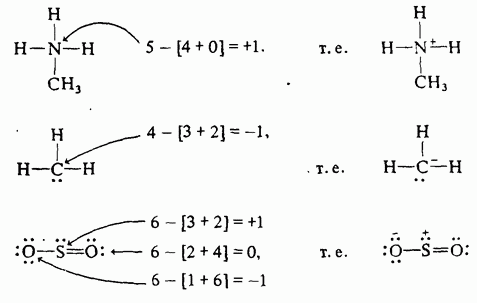
\includegraphics[width=0.7\linewidth]{7.example}
	\caption{Пример определения формального заряда атома в соединении с помощью структур Льюиса}
	\label{fig:7.example}
\end{figure}






